\documentclass[12pt,a4paper]{article}

% ==========================================================
% CONFIGURACIÓN GENERAL
% ==========================================================
\usepackage[utf8]{inputenc}
\usepackage[T1]{fontenc}
\usepackage[spanish,es-tabla]{babel}

\usepackage[
    a4paper,
    top=2.8cm,
    bottom=2.5cm,
    left=2.5cm,
    right=2.5cm,
    headheight=80pt
]{geometry}

% ==========================================================
% PAQUETES
% ==========================================================
\usepackage{lmodern}
\usepackage{amsmath}
\usepackage{amssymb}
\usepackage{graphicx}
\usepackage{xcolor}
\usepackage{float}
\usepackage{booktabs}
\usepackage{tabularx}
\usepackage{array}
\usepackage{enumitem}
\usepackage{multicol}
\usepackage{subcaption}
\usepackage{fancyhdr}
\usepackage{listings}
\usepackage{hyperref}
\usepackage{microtype}
\usepackage{longtable}

% Color utilizado en las listas
\definecolor{accentblue}{RGB}{31,78,121}
\definecolor{codegray}{rgb}{0.5,0.5,0.5}
\definecolor{backcolour}{rgb}{0.96,0.96,0.96}

% Configuración de listings para código Python
\lstdefinestyle{mystyle}{
    backgroundcolor=\color{backcolour},   
    commentstyle=\color{codegray}\itshape,
    keywordstyle=\color{accentblue}\bfseries,
    numberstyle=\tiny\color{codegray},
    basicstyle=\ttfamily\footnotesize,
    breakatwhitespace=false,         
    breaklines=true,                 
    captionpos=b,                    
    keepspaces=true,                 
    numbers=left,                    
    numbersep=5pt,                  
    showspaces=false,                
    showstringspaces=false,
    showtabs=false,                  
    tabsize=2
}
\lstset{style=mystyle}

% ==========================================================
% CONFIGURACIÓN DE HYPERREF
% ==========================================================
\hypersetup{
    colorlinks=true,
    linkcolor=black,
    filecolor=black,
    urlcolor=blue,
    citecolor=black,
    pdftitle={Ecualización Manual de Histogramas RGB y Ajuste de Luminosidad},
    pdfauthor={Marlon Guevara - Jonathan Fiallos}
}

% ==========================================================
% COMANDO PARA CHECKBOX
% ==========================================================
\newcommand{\checkedbox}{\boxtimes}

% ==========================================================
% ENCABEZADO Y PIE DE PÁGINA
% ==========================================================
\pagestyle{fancy}
\fancyhf{}

\fancyhead[C]{%
    \begin{minipage}[c]{2.5cm}
        \centering
        
\includegraphics[width=1.3cm]{imagenes/uta.png}
    \end{minipage}%
    \hfill
    \begin{minipage}[c]{9.5cm}
        \centering
        \small \textbf{UNIVERSIDAD TÉCNICA DE AMBATO}\\[0.1cm]
        \scriptsize \textit{
        FACULTAD DE INGENIERÍA EN SISTEMAS,
        ELECTRÓNICA E INDUSTRIAL}\\[0.1cm]
        \scriptsize \textbf{CARRERA DE SOFTWARE}\\[0.1cm]
        \scriptsize \textbf{CICLO ACADÉMICO: AGOSTO -- DICIEMBRE 2026}
    \end{minipage}%
    \hfill
    \begin{minipage}[c]{2.5cm}
        \centering
        
\includegraphics[width=1.3cm]{imagenes/fisei.png}
    \end{minipage}%
}

\fancyfoot[C]{\thepage}

% ==========================================================
% INICIO DEL DOCUMENTO
% ==========================================================
\begin{document}

% ==========================================================
% PORTADA
% ==========================================================
\begin{center}

\vspace*{0.8cm}

{\Large \textbf{UNIVERSIDAD TÉCNICA DE AMBATO}}

\vspace{0.3cm}

{\large
\textbf{FACULTAD DE INGENIERÍA EN SISTEMAS,
ELECTRÓNICA E INDUSTRIAL}}

\vspace{0.3cm}

{\large \textbf{CARRERA DE SOFTWARE}}

\vspace{1.2cm}


\includegraphics[width=3.8cm]{imagenes/uta.png}

\vspace{1.0cm}

{\Large \textbf{INFORME DE GUÍA PRÁCTICA (APE)}}

\vspace{0.8cm}

{\large
\textbf{APE. Procesamiento Digital de Imágenes: Ecualización Manual de Histogramas en Canales RGB y Corrección Gamma de Luminosidad sin Librerías Especializadas}}

\vspace{1.2cm}

\begin{flushleft}

\textbf{Unidad de Organización Curricular:}
Profesional

\vspace{0.2cm}

\textbf{Asignatura:}
Procesamiento de Imágenes

\vspace{0.4cm}

\textbf{Alumnos participantes:}

\begin{itemize}
    \item Guevara Panimboza Marlon Steven
    \item Fiallos Yanza Jonathan Josue 
\end{itemize}

\end{flushleft}

\vfill

\textbf{Ambato -- Ecuador}

\textbf{Agosto -- Diciembre 2026}

\end{center}

\newpage

% ==========================================================
% ÍNDICE
% ==========================================================
\tableofcontents

\newpage

% ==========================================================
% I. TEMA
% ==========================================================
\section{Tema}

Desarrollo, Implementación y Análisis Matemático de la Ecualización Manual de Histogramas Canal por Canal en Imágenes RGB y Corrección Gamma de Luminosidad mediante Algoritmos Artesanales en Python.

% ==========================================================
% II. OBJETIVO
% ==========================================================
\section{Objetivo}

Diseñar, implementar y evaluar el algoritmo de ecualización de histograma de forma completamente manual (sin librerías de caja negra como \texttt{cv2.equalizeHist} o \texttt{skimage.exposure}), aplicándolo a cada uno de los canales del modelo cromático RGB (Rojo, Verde y Azul) y extendiendo el procedimiento al ajuste de luminosidad por transformación no lineal (gamma), con el propósito de:

\begin{enumerate}[label=\alph*)]
    \item Descomponer la imagen en sus planos matriciales de intensidad fundamentales y calcular de forma determinista su función de frecuencia discreta (histograma).
    \item Calcular rigurosamente la función de densidad de probabilidad discretizada (PDF) y la función de distribución acumulada (CDF).
    \item Construir las tablas de consulta directa (\textit{Look-Up Table}, LUT) para el mapeo determinista de intensidades de 8 bits ($0 \dots 255$).
    \item Demostrar analítica y visualmente el efecto de desplazamiento cromático (\textit{color shift}) resultante de la ecualización desacoplada en el espacio RGB.
    \item Replicar en Python la funcionalidad de las directivas clásicas de MATLAB (\texttt{histeq}, \texttt{imadjust}, \texttt{cat(3,...)}) mediante lógica vectorizada en NumPy.
\end{enumerate}

% ==========================================================
% III. MODALIDAD
% ==========================================================
\section{Modalidad}

Presencial / Práctica de Laboratorio y Análisis Numérico.

% ==========================================================
% IV. TIEMPO DE DURACIÓN
% ==========================================================
\section{Tiempo de duración}

\begin{itemize}
    \item Presenciales: 4 horas.
    \item No presenciales: 2 horas.
\end{itemize}

% ==========================================================
% V. INSTRUCCIONES
% ==========================================================
\section{Instrucciones}

Para el correcto desarrollo de la práctica se adoptan las siguientes directrices metodológicas:

\begin{itemize}
    \item Utilizar una imagen digital en color de alta definición en formato JPEG (\texttt{High Res Wallpaper HD.jpg}) de dimensiones conocidas.
    \item Prohibir taxativamente el uso de módulos o funciones automáticas de ecualización de histograma provenientes de OpenCV, Scikit-Image o SciPy.
    \item Estructurar el código en celdas reproducibles dentro de un cuaderno Jupyter Notebook interactivo (\texttt{ecualizacion\_rgb\_manual.ipynb}).
    \item Implementar el conteo de frecuencias de los niveles $0 \dots 255$ directamente sobre los arreglos bidimensionales de cada canal.
    \item Presentar los canales individuales en dos modalidades visuales: escala de grises (magnitud de intensidad escalar) y en color aislado (proyección vectorial tridimensional RGB con los otros dos planos en cero).
    \item Extraer y graficar las curvas características de transformación acumulativa (LUT) comparadas contra la recta de identidad.
    \item Realizar el ensamblado de los tres canales transformados para comparar la imagen original frente a la ecualizada.
    \item Implementar la corrección gamma manual para simular el comportamiento de \texttt{imadjust} y diseñar una interfaz de controles deslizantes dinámicos (\texttt{ipywidgets}).
\end{itemize}

% ==========================================================
% VI. EQUIPOS Y RECURSOS
% ==========================================================
\section{Listado de equipos, materiales y recursos}

\textbf{Listado de equipos y materiales empleados:}

\begin{itemize}
    \item Computador personal con arquitectura x86\_64 y sistema operativo Microsoft Windows.
    \item Entorno de ejecución interactivo Jupyter Notebook con núcleo Python 3.12.
    \item Librerías matemáticas y de graficación:
    \begin{itemize}
        \item \textbf{NumPy:} Álgebra lineal, manipulación matricial multidimensional y operaciones vectorizadas.
        \item \textbf{Matplotlib (PyPlot):} Trazado de histogramas discretos, subgráficas comparativas y visualización raster.
        \item \textbf{Pillow (PIL):} Empleada exclusivamente para la lectura inicial y conversión a arreglo RGB.
        \item \textbf{IPyWidgets:} Deslizadores interactivos para parametrización en tiempo real.
    \end{itemize}
    \item Sistema de tipografía técnica \LaTeX{} bajo la distribución MiKTeX.
\end{itemize}

\textbf{TAC (Tecnologías para el Aprendizaje y Conocimiento) empleadas:}

\begin{itemize}
    \item[$\checkedbox$] Entornos de desarrollo interactivos (Jupyter / VS Code).
    \item[$\checkedbox$] Software de cálculo simbólico y numérico.
    \item[$\checkedbox$] Procesamiento digital de señales e imágenes.
    \item[$\square$] Recursos audiovisuales.
    \item[$\checkedbox$] Inteligencia Artificial y modelado algorítmico.
\end{itemize}

% ==========================================================
% VII. ACTIVIDADES POR DESARROLLAR
% ==========================================================
\section{Actividades por desarrollar}

El desarrollo se fundamenta en los principios formales del procesamiento espacial de imágenes monocromáticas y policromáticas, articulado en las siguientes fases:

\subsection{Fundamento Matemático del Histograma Digital}

Sea una imagen digital discreta definida como una función bidimensional de intensidad $f(x, y)$, donde $x \in \{0, 1, \dots, M-1\}$ e $y \in \{0, 1, \dots, N-1\}$. La imagen está compuesta por un total de $N_{total} = M \times N$ píxeles. La intensidad de cada píxel está cuantizada en $L$ niveles discretos en el rango $[0, L-1]$, donde para imágenes de 8 bits por canal, $L = 256$ (niveles enteros de $0$ a $255$).

El \textbf{histograma no normalizado} $h(r_k)$ de un canal representa la frecuencia absoluta con la que el nivel de intensidad $r_k = k$ aparece en la matriz:

\begin{equation}
h(r_k) = n_k = \sum_{x=0}^{M-1} \sum_{y=0}^{N-1} \delta(f(x, y) - k), \quad \text{para } k = 0, 1, \dots, L-1
\end{equation}

donde $\delta(\cdot)$ es la función delta de Kronecker:

\begin{equation}
\delta(u) = \begin{cases} 
1 & \text{si } u = 0 \\
0 & \text{si } u \neq 0 
\end{cases}
\end{equation}

\subsection{Normalización y Función de Densidad de Probabilidad (PDF)}

Dividiendo cada frecuencia absoluta entre el número total de píxeles $N_{total}$, se obtiene el histograma normalizado o \textbf{Función de Densidad de Probabilidad} discretizada (PDF, por sus siglas en inglés):

\begin{equation}
p_r(r_k) = \frac{n_k}{N_{total}} = \frac{h(r_k)}{\sum_{j=0}^{L-1} n_j}
\end{equation}

Dicha función satisface axiomáticamente las propiedades de una distribución de probabilidad discreta:

\begin{equation}
0 \le p_r(r_k) \le 1 \quad \forall k, \qquad \sum_{k=0}^{L-1} p_r(r_k) = 1.0
\end{equation}

\subsection{Función de Distribución Acumulada (CDF)}

La \textbf{Función de Distribución Acumulada} (CDF) de los niveles de intensidad corresponde a la suma acumulada de las probabilidades desde el nivel inicial $0$ hasta el nivel $k$:

\begin{equation}
CDF[k] = P(r \le r_k) = \sum_{j=0}^{k} p_r(r_j) = \frac{1}{N_{total}} \sum_{j=0}^{k} n_j
\end{equation}

Esta función es monótonamente no decreciente en el intervalo $[0, 1]$:

\begin{equation}
CDF[0] = p_r(0), \qquad CDF[L-1] = 1.0, \qquad CDF[k] \ge CDF[k-1]
\end{equation}

\subsection{Transformación de Ecualización y Construcción de la Tabla LUT}

El principio teórico de la ecualización de histograma busca encontrar una función de transformación monotónica $s_k = T(r_k)$ tal que la variable aleatoria transformada $s$ posea una distribución de probabilidad lo más uniforme posible en el intervalo completo de salida $[0, L-1]$.

En el dominio discreto, incorporando la compensación del primer valor acumulado no nulo $CDF_{min} = \min_{k}\{CDF[k] \mid CDF[k] > 0\}$ para asegurar el estiramiento completo desde el nivel cero, se aplica la ecuación canónica:

\begin{equation}
LUT[k] = \text{round}\left( \frac{CDF[k] - CDF_{min}}{1.0 - CDF_{min}} \times (L - 1) \right)
\end{equation}

Posteriormente, se satura formalmente el valor en el espacio entero $\mathbb{N}_0$:

\begin{equation}
LUT[k] = \max\Big(0, \min\big(255, LUT[k]\big)\Big) \in [0, 255]
\end{equation}

\subsection{Aplicación por Indexación Directa (Mapeo Espacial)}

Una vez precalculada la tabla unidimensional $LUT$ de tamaño $256$, la ecualización de cada píxel de la matriz $f(x, y)$ se realiza en tiempo constante $\mathcal{O}(1)$ por reindexación de memoria:

\begin{equation}
g(x, y) = LUT\big[ f(x, y) \big]
\end{equation}

Este procedimiento se ejecuta de manera independiente para cada uno de los tres canales del espacio RGB:
\begin{align}
R_{ecualizado}(x, y) &= LUT_R\big[ R(x, y) \big] \\
G_{ecualizado}(x, y) &= LUT_G\big[ G(x, y) \big] \\
B_{ecualizado}(x, y) &= LUT_B\big[ B(x, y) \big]
\end{align}

\subsection{Corrección Gamma de Luminosidad (Equivalente a \texttt{imadjust})}

En MATLAB, la instrucción \texttt{imadjust(I, [], [], 1/luminosidad)} aplica una corrección de potencia gamma no lineal sobre la escala normalizada $[0, 1]$. La ecuación matemática que modela este ajuste sobre cada píxel $p \in [0, 255]$ es:

\begin{equation}
p_{salida} = 255 \cdot \left( \frac{p_{entrada}}{255.0} \right)^{\frac{1}{\gamma}}
\end{equation}

\begin{itemize}
    \item Para $\gamma > 1.0$: La función es convexa, elevando los valores de los tonos medios y oscuros, produciendo un incremento global de \textbf{luminosidad y claridad}.
    \item Para $\gamma < 1.0$: La función es cóncava, comprimiendo los niveles altos y acentuando las sombras, produciendo un efecto de \textbf{oscurecimiento}.
\end{itemize}

\subsection{Equivalencia Funcional MATLAB vs. Implementación Python}

La Tabla~\ref{tab:equivalencia_matlab} sintetiza la correlación directa entre los comandos nativos de MATLAB y la solución algorítmica artesanal construida en Python:

\begin{table}[H]
\centering
\caption{Equivalencia metodológica entre directivas MATLAB y Python manual}
\label{tab:equivalencia_matlab}
\renewcommand{\arraystretch}{1.25}
\footnotesize
\begin{tabularx}{\textwidth}{p{3.2cm}p{5.5cm}X}
\toprule
\textbf{Operación} & \textbf{MATLAB (\textit{Toolbox})} & \textbf{Python Artesanal (NumPy / PIL)} \\
\midrule
Lectura de imagen & \texttt{I = imread('foto.jpg');} & \texttt{np.array(Image.open(...))} \\
Separación de canales & \texttt{R = I(:,:,1); G=I(:,:,2); B=I(:,:,3);} & \texttt{R, G, B = img[:,:,0], img[:,:,1], img[:,:,2]} \\
Cálculo de histograma & \texttt{h = imhist(canal);} & \texttt{histograma\_manual(canal)} vía conteo \\
Ecualización & \texttt{eq = histeq(canal);} & \texttt{lut[canal]} derivado de $CDF$ paso a paso \\
Unión cromática & \texttt{unida = cat(3, R, G, B);} & \texttt{np.stack([redEq, greenEq, blueEq], axis=2)} \\
Ajuste gamma & \texttt{imadjust(I, [], [], 1/lum);} & \texttt{np.clip(((x/255)**(1/lum))*255, 0, 255)} \\
Visualización múltiple & \texttt{subplot(m, n, p); imshow(...);} & \texttt{plt.subplots(...); ax.imshow(...)} \\
\bottomrule
\end{tabularx}
\end{table}

% ==========================================================
% VIII. RESULTADOS OBTENIDOS
% ==========================================================
\section{Resultados obtenidos}

A continuación, se documenta la experimentación efectuada sobre la imagen de prueba \texttt{High Res Wallpaper HD.jpg}, detallando los resultados cuantitativos y cualitativos obtenidos en cada fase.

\subsection{Caracterización de la Imagen de Entrada}

La imagen empleada en la práctica posee las siguientes propiedades estructurales:
\begin{itemize}
    \item \textbf{Dimensiones de la matriz:} $414$ píxeles de alto por $736$ píxeles de ancho.
    \item \textbf{Canales cromáticos:} $3$ planos ortogonales (Rojo, Verde, Azul).
    \item \textbf{Población total de píxeles:} $N_{total} = 414 \times 736 = 304{,}704$ píxeles.
    \item \textbf{Profundidad de color:} 8 bits sin signo (\texttt{uint8}), correspondiente a valores enteros en el intervalo $[0, 255]$.
\end{itemize}

En la Figura~\ref{fig:original} se presenta la imagen digital original previo a cualquier procesamiento espacial.

\begin{figure}[H]
\centering
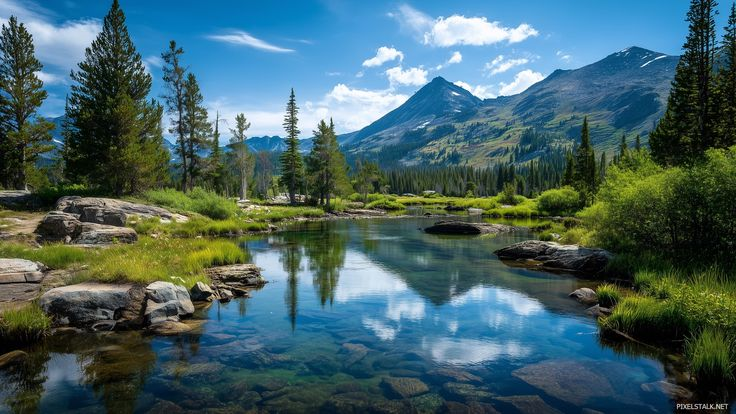
\includegraphics[width=0.70\textwidth]{imagenes/imagen_original.png}
\caption{Imagen digital original (\texttt{High Res Wallpaper HD.jpg}) de $414 \times 736$ píxeles.}
\label{fig:original}
\end{figure}

\subsection{Análisis Estadístico de Canales Iniciales}

La evaluación numérica de la media ($\mu$) y desviación estándar ($\sigma$) de los niveles de intensidad para cada canal arrojó los siguientes valores cuantitativos:

\begin{itemize}
    \item \textbf{Canal Rojo ($R$):} Mínimo = $0$, Máximo = $255$, Media $\mu_R = 68.81$, Desviación $\sigma_R = 53.78$.
    \item \textbf{Canal Verde ($G$):} Mínimo = $0$, Máximo = $255$, Media $\mu_G = 98.86$, Desviación $\sigma_G = 57.83$.
    \item \textbf{Canal Azul ($B$):} Mínimo = $0$, Máximo = $255$, Media $\mu_B = 102.17$, Desviación $\sigma_B = 78.12$.
\end{itemize}

\subsection{Descomposición de Canales y Respuesta del Canal Azul}

Uno de los aspectos analíticos más relevantes de la práctica radica en la correcta descomposición e interpretación del canal Azul:

\begin{enumerate}
    \item \textbf{Aislamiento riguroso del canal:} Al indexar \texttt{B = img[:, :, 2]}, se extrae pura y exclusivamente la intensidad azul del arreglo tridimensional. No existe mezcla con rojo ni verde.
    \item \textbf{Modalidad en escala de grises vs. color aislado:} 
    \begin{itemize}
        \item Cuando el canal se grafica en escala de grises (\texttt{cmap='gray'}), los píxeles claros representan altas intensidades de azul y los oscuros ausencia de radiación azul.
        \item Cuando se proyecta en color aislado (\texttt{solo\_canal(B, 2)}), se genera la tupla vectorial $[0, 0, B(x, y)]$, cancelando las longitudes de onda roja y verde.
    \end{itemize}
    \item \textbf{Comportamiento del histograma azul:} El histograma del canal azul presenta una alta concentración de niveles por encima de $150$, explicando por qué visualmente el cielo y las zonas abiertas exhiben un tono azul saturado.
\end{enumerate}

La Figura~\ref{fig:canales_antes} ilustra de manera sinóptica la descomposición inicial de los tres canales en sus representaciones de intensidad pura (escala de grises), plano cromático aislado (RGB) y sus respectivos histogramas reales.

\begin{figure}[H]
\centering
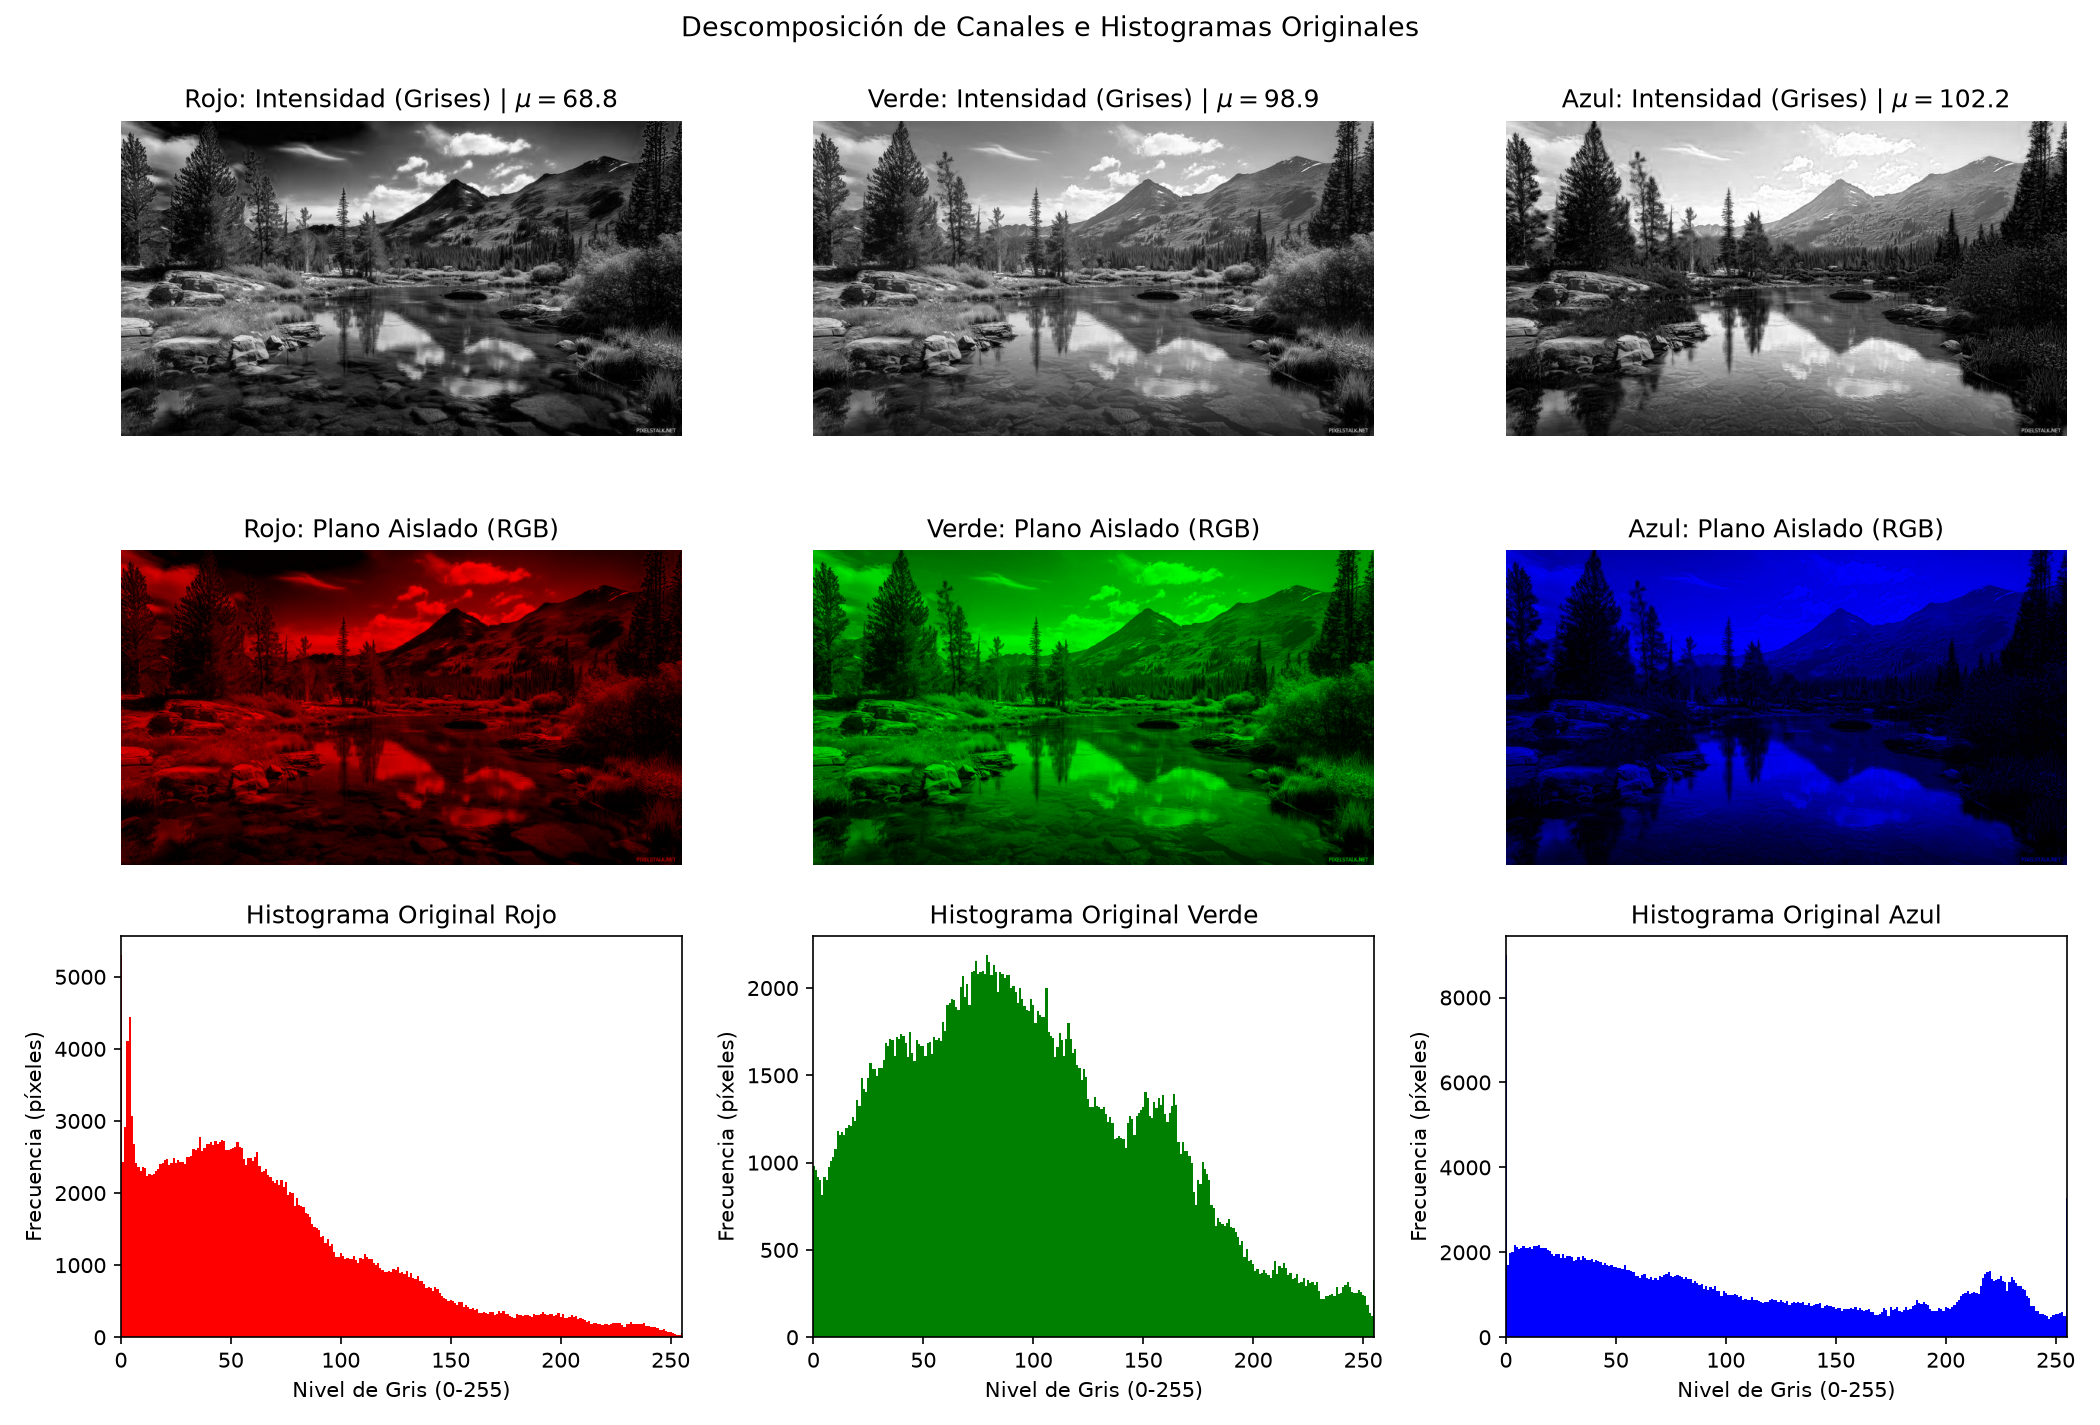
\includegraphics[width=\textwidth]{imagenes/canales_antes.png}
\caption{Descomposición inicial de canales antes de la ecualización: Fila 1 (Intensidad en escala de grises), Fila 2 (Plano de color aislado en RGB), Fila 3 (Histograma de frecuencia real).}
\label{fig:canales_antes}
\end{figure}

\subsection{Cálculo Numérico Paso a Paso y Verificación de Tablas LUT}

En la Tabla~\ref{tab:muestreo_lut} se documenta una muestra representativa de los cálculos matemáticos efectuados por el algoritmo manual para distintos niveles de entrada $k \in \{0, 50, 100, 150, 200, 255\}$, permitiendo auditar la coherencia de la transformación:

\begin{table}[H]
\centering
\caption{Auditoría matemática de frecuencias, probabilidades acumuladas y valores transformados}
\label{tab:muestreo_lut}
\renewcommand{\arraystretch}{1.2}
\resizebox{\textwidth}{!}{%
\begin{tabular}{c|ccc|ccc|ccc}
\toprule
\textbf{Nivel} & \multicolumn{3}{c|}{\textbf{Canal Rojo ($R$)}} & \multicolumn{3}{c|}{\textbf{Canal Verde ($G$)}} & \multicolumn{3}{c}{\textbf{Canal Azul ($B$)}} \\
\textbf{Entrada} $k$ & $h_R[k]$ & $CDF_R[k]$ & $LUT_R[k]$ & $h_G[k]$ & $CDF_G[k]$ & $LUT_G[k]$ & $h_B[k]$ & $CDF_B[k]$ & $LUT_B[k]$ \\
\midrule
0   & 381  & 0.0013 & \textbf{0}   & 472  & 0.0015 & \textbf{0}   & 518  & 0.0017 & \textbf{0}   \\
50  & 2607 & 0.4431 & \textbf{110} & 1667 & 0.2324 & \textbf{59}  & 1656 & 0.3457 & \textbf{83}  \\
100 & 1169 & 0.7660 & \textbf{194} & 1903 & 0.5521 & \textbf{140} & 1045 & 0.5704 & \textbf{142} \\
150 & 514  & 0.9112 & \textbf{232} & 1319 & 0.7927 & \textbf{202} & 665  & 0.7077 & \textbf{178} \\
200 & 274  & 0.9681 & \textbf{247} & 421  & 0.9449 & \textbf{241} & 716  & 0.8169 & \textbf{207} \\
255 & 48   & 1.0000 & \textbf{255} & 18   & 1.0000 & \textbf{255} & 61   & 1.0000 & \textbf{255} \\
\bottomrule
\end{tabular}%
}
\end{table}

\textbf{Análisis de la tabla de transformación:}
\begin{itemize}
    \item En el canal Rojo, el nivel de entrada $50$ alcanza un $CDF = 0.4431$, por lo cual se proyecta al nivel de salida $110$, sufriendo un incremento de $+60$ niveles de brillo. Esto se debe a que más del $44\%$ de los píxeles rojos estaban concentrados en tonos oscuros.
    \item Por el contrario, en el canal Verde, el nivel $50$ solo acumula un $23.24\%$ de la masa probabilística, por lo que su salida mapeada es de $59$ (apenas $+9$ niveles de variación).
    \item Esta marcada diferencia en las pendientes de transferencia genera las tres curvas diferenciales mostradas en la Figura~\ref{fig:curvas_lut}.
\end{itemize}

\begin{figure}[H]
\centering
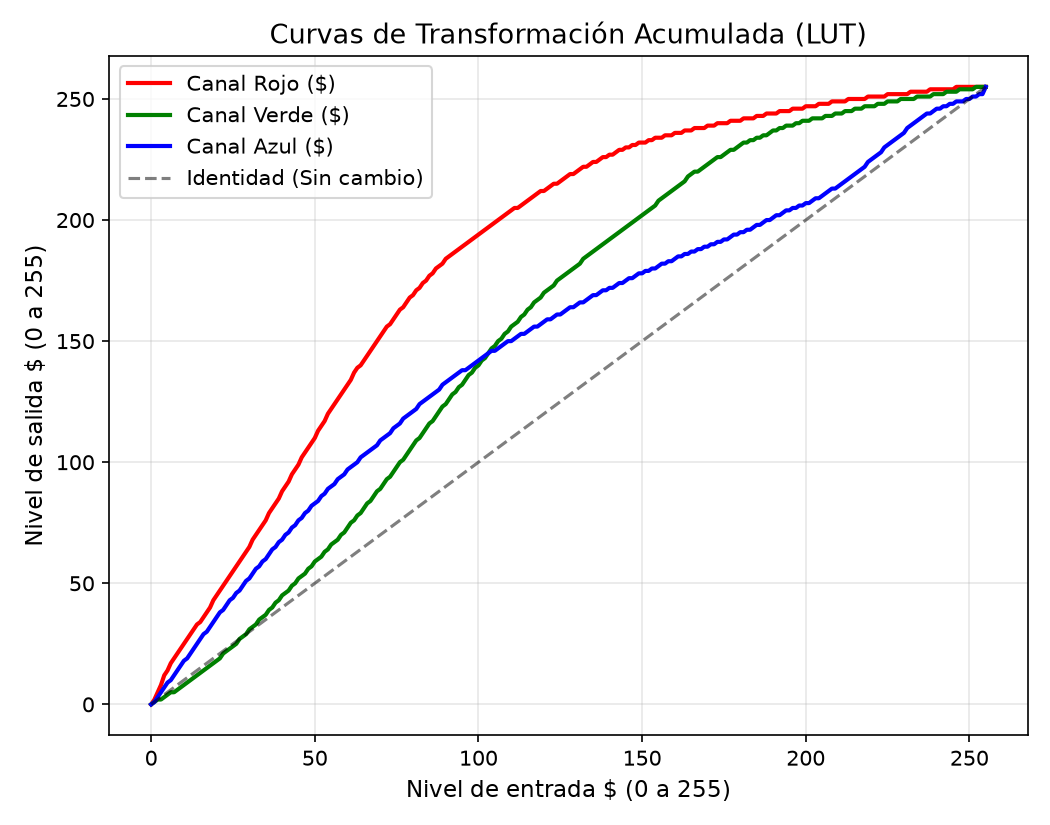
\includegraphics[width=0.68\textwidth]{imagenes/curvas_lut.png}
\caption{Curvas de transformación acumulada ($LUT$) para cada canal cromático frente a la diagonal de identidad (sin alteración).}
\label{fig:curvas_lut}
\end{figure}

\subsection{Evaluación de Canales tras la Ecualización}

Tras aplicar las tres tablas $LUT$ de manera vectorizada, los histogramas de los canales individuales se aplanan notablemente, distribuyendo las frecuencias de manera uniforme a lo largo del intervalo completo $[0, 255]$, tal como se ilustra en la Figura~\ref{fig:canales_despues}.

\begin{figure}[H]
\centering
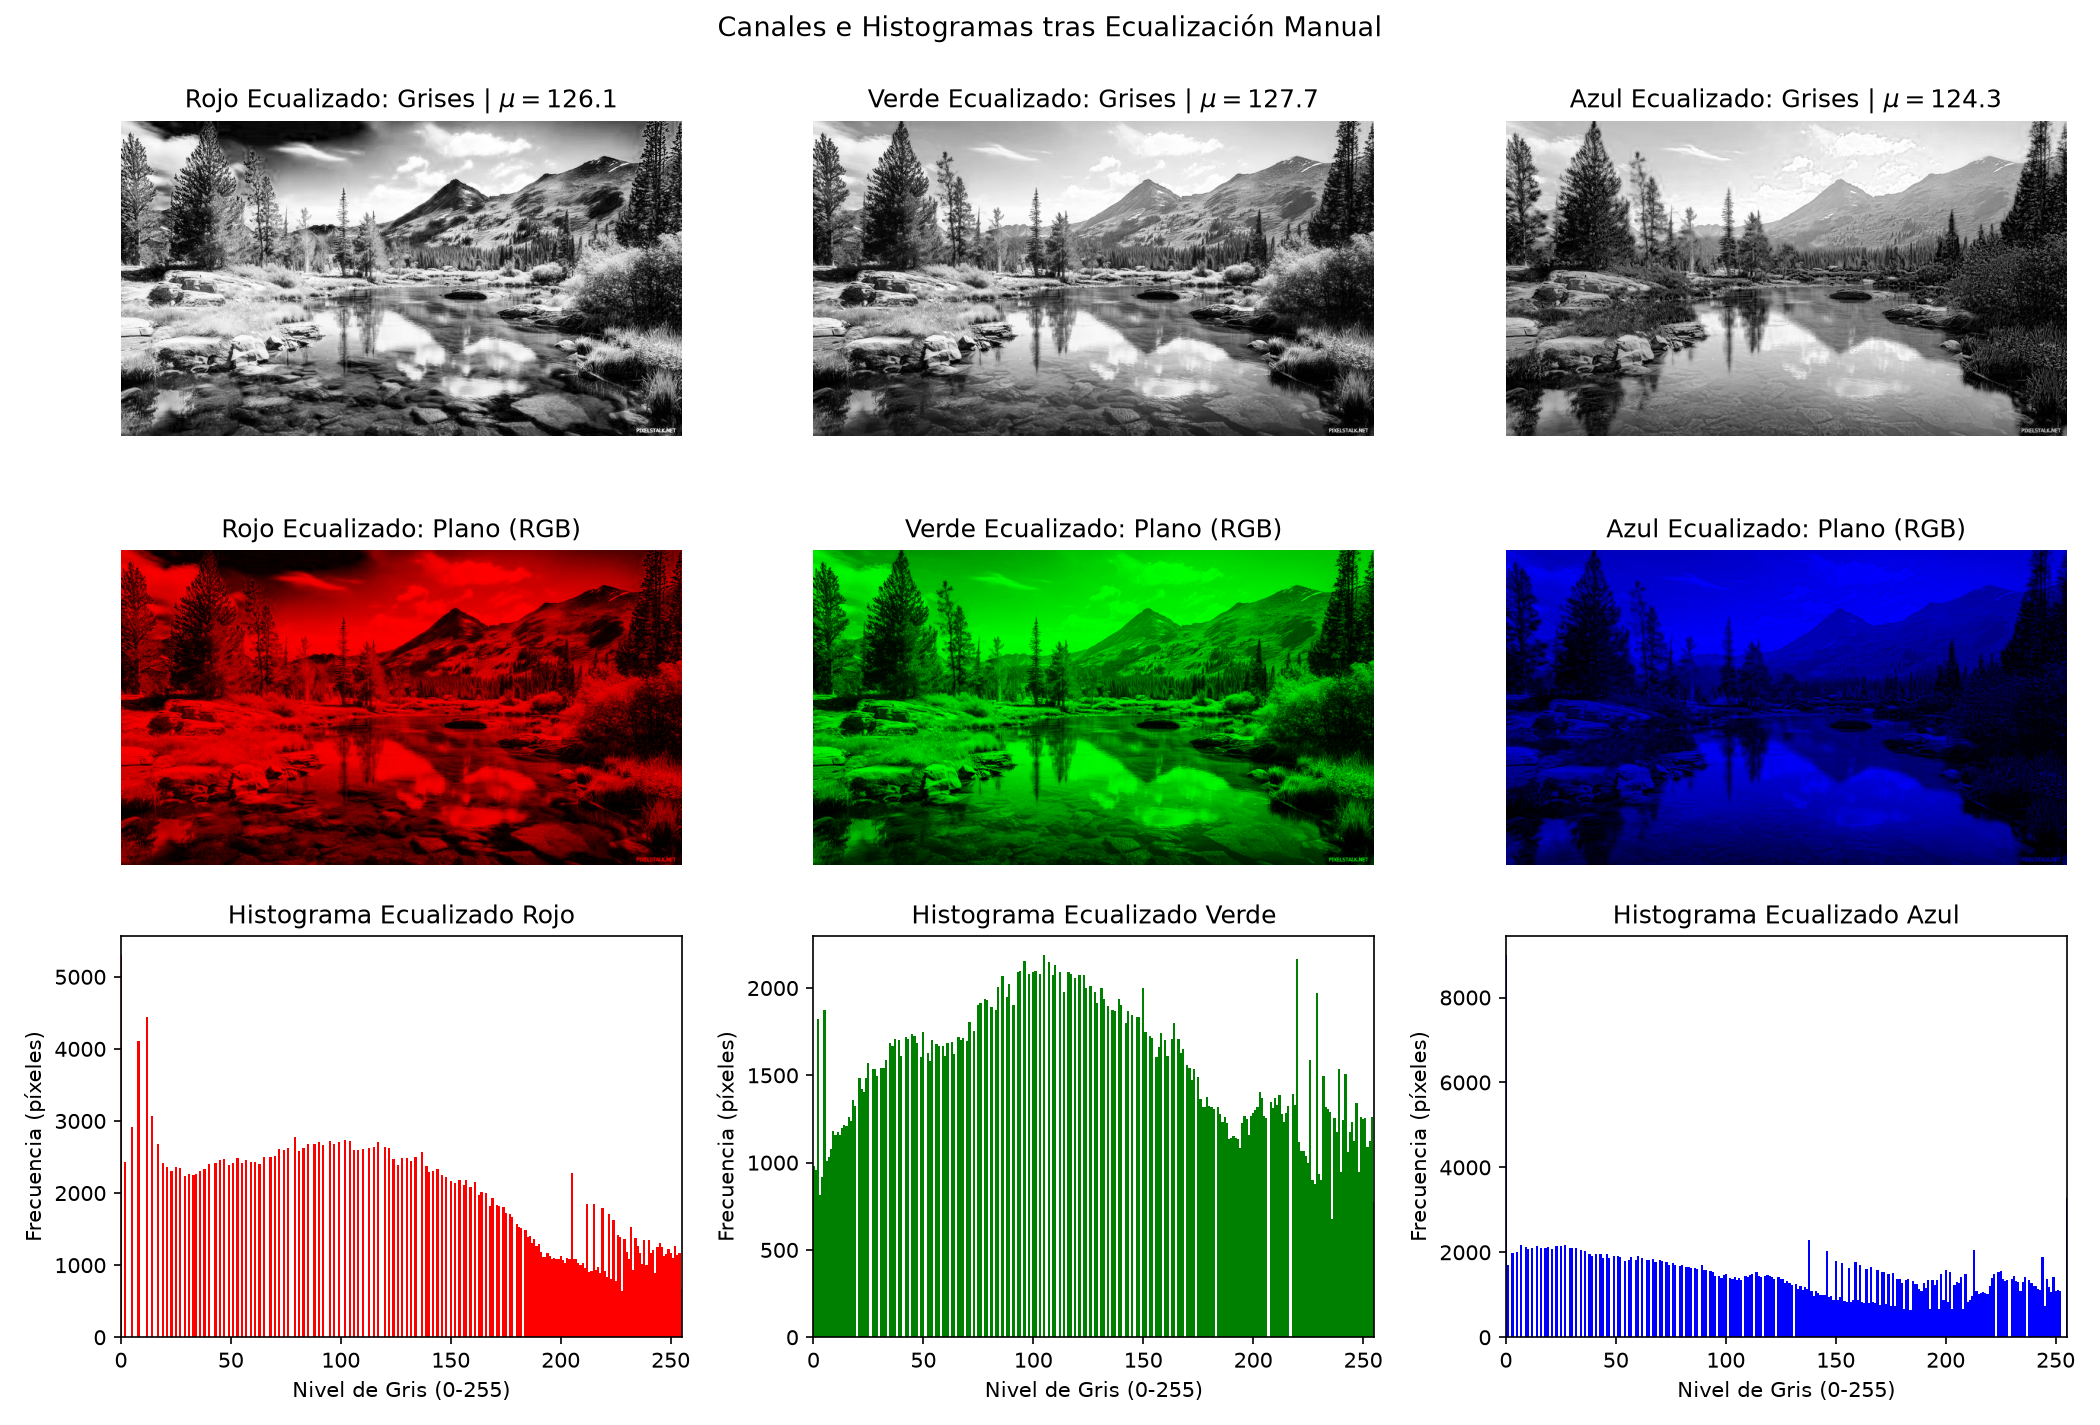
\includegraphics[width=\textwidth]{imagenes/canales_despues.png}
\caption{Canales e histogramas resultantes tras la ecualización manual: la densidad de probabilidad se redistribuye a lo largo de todo el espectro dinámico.}
\label{fig:canales_despues}
\end{figure}

La Figura~\ref{fig:comparacion_histogramas} complementa la visualización mediante una comparativa directa con áreas rellenas superpuestas (histograma original en gris versus histograma ecualizado en color), confirmando la expansión del contraste.

\begin{figure}[H]
\centering
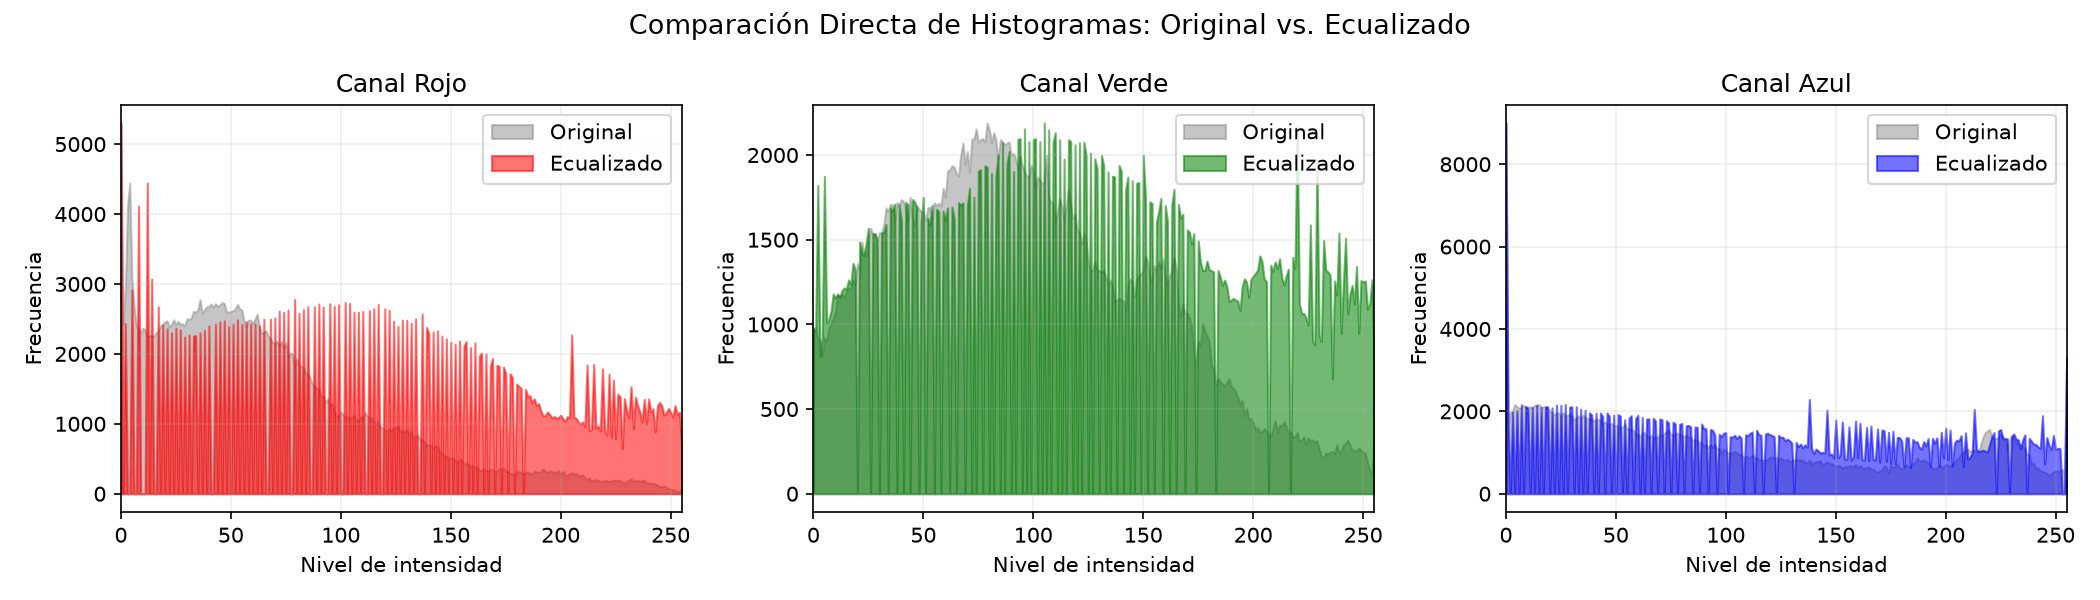
\includegraphics[width=\textwidth]{imagenes/comparacion_histogramas.png}
\caption{Comparativa directa superpuesta de histogramas antes (área gris) y después de la ecualización manual.}
\label{fig:comparacion_histogramas}
\end{figure}

\subsection{Reconstrucción Cromática y Fenómeno de Desplazamiento de Color (\textit{Color Shift})}

Al concatenar los canales resultantes mediante \texttt{np.stack([redEq, greenEq, blueEq], axis=2)}, equivalente a la operación \texttt{cat(3, ...)} de MATLAB, se obtiene la imagen final ecualizada en RGB, ilustrada en la Figura~\ref{fig:comparacion_rgb}.

\begin{figure}[H]
\centering
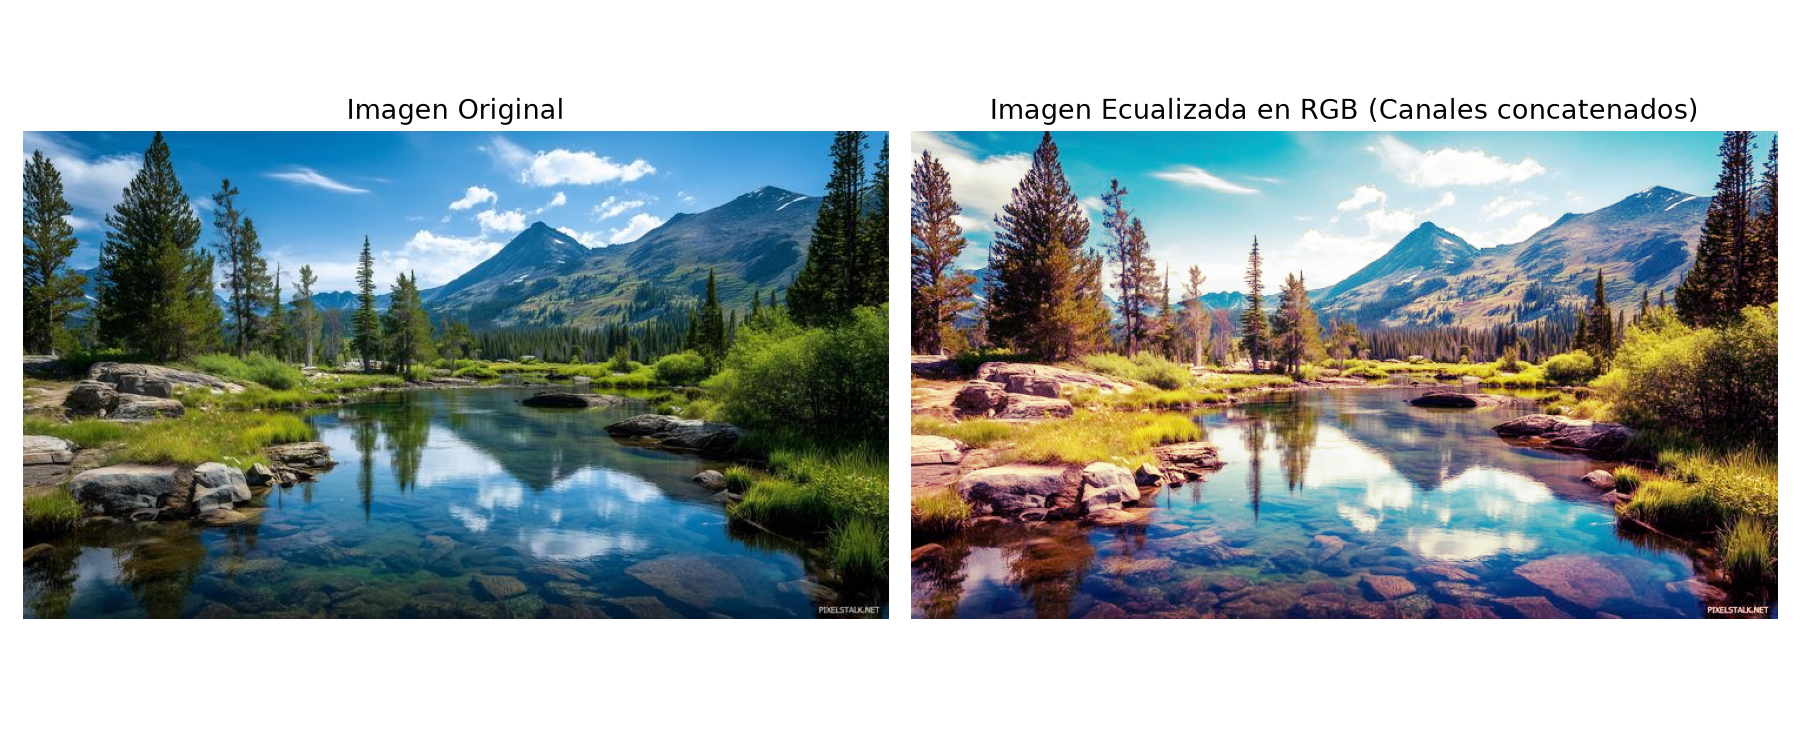
\includegraphics[width=\textwidth]{imagenes/comparacion_rgb.png}
\caption{Comparación final: Imagen original (izquierda) frente a imagen ecualizada por canales independientes en RGB (derecha).}
\label{fig:comparacion_rgb}
\end{figure}

\textbf{Discusión teórica fundamental sobre la alteración cromática:}
\begin{itemize}
    \item Se observa de forma contundente que la imagen ecualizada en RGB presenta un fuerte \textbf{desplazamiento cromático} (\textit{color shift}), alterando la tonalidad natural de la escena.
    \item \textbf{Causa matemática:} En el espacio tridimensional RGB, las variables $R, G, B$ están correlacionadas intrínsecamente tanto con la luminancia como con la crominancia. Las razones de cromaticidad originales:
    \begin{equation}
    r = \frac{R}{R+G+B}, \qquad g = \frac{G}{R+G+B}, \qquad b = \frac{B}{R+G+B}
    \end{equation}
    son severamente modificadas porque cada canal sufre una función de transformación $LUT$ diferente. Por ejemplo, un píxel original con proporciones $1 : 1.5 : 2$ pasa a tener proporciones desbalanceadas, provocando saturación artificial y tintes azulados o rojizos.
    \item \textbf{Solución en la industria profesional:} En procesamiento avanzado de imágenes, para evitar la alteración del color se transforma la imagen al espacio de color \textbf{HSV} o \textbf{CIE-Lab}, donde se ecualiza \textbf{únicamente el canal de brillo/luminancia} ($V$ o $L$), preservando el tono ($H$) y la saturación ($S$) intactos.
\end{itemize}

\subsection{Ajuste no Lineal de Luminosidad por Corrección Gamma}

Finalmente, se aplicó la corrección gamma manual sobre la imagen ecualizada unida utilizando un parámetro de luminosidad $\gamma = 1.2$. La Figura~\ref{fig:ajuste_gamma} evidencia cómo la curva potencial aclara suavemente las regiones de penumbra sin saturar los picos de altas luces.

\begin{figure}[H]
\centering
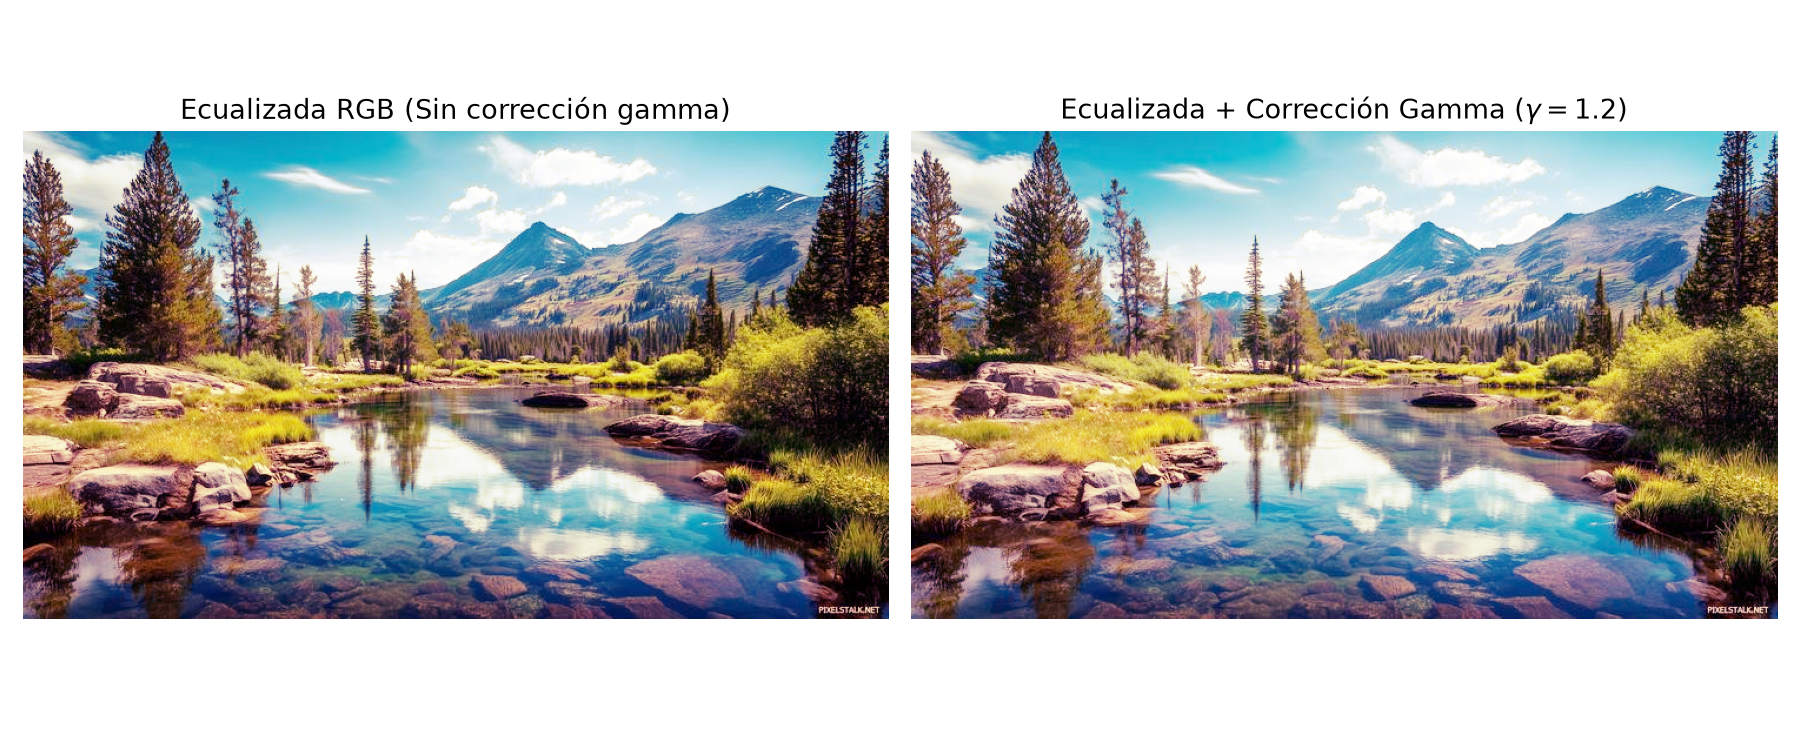
\includegraphics[width=\textwidth]{imagenes/ajuste_luminosidad.png}
\caption{Ajuste de luminosidad gamma: Imagen ecualizada sin corrección (izquierda) frente a la imagen con corrección gamma $\gamma = 1.2$ (derecha).}
\label{fig:ajuste_gamma}
\end{figure}

% ==========================================================
% IX. HABILIDADES BLANDAS
% ==========================================================
\section{Habilidades blandas empleadas en la práctica}

\begin{itemize}
    \item[$\checkedbox$] \textbf{Resolución de problemas complejos:} Deducción e implementación manual de modelos probabilísticos sin recurrir a funciones prefabricadas.
    \item[$\checkedbox$] \textbf{Pensamiento analítico y crítico:} Identificación de las limitaciones inherentes a la ecualización en el espacio de color RGB frente a espacios desacoplados.
    \item[$\checkedbox$] \textbf{Trabajo colaborativo y rigor metodológico:} Coordinación en la depuración del código, contrastación de resultados experimentales y redacción formal del reporte técnico.
\end{itemize}

% ==========================================================
% X. CONCLUSIONES
% ==========================================================
\section{Conclusiones}

\begin{itemize}[leftmargin=1.2cm]
    \item Se implementó con éxito el algoritmo completo de ecualización de histograma de forma 100\% artesanal en Python, verificando que el uso de la función de probabilidad acumulada discretizada ($CDF$) normalizada con corrección de $CDF_{min}$ garantiza el aprovechamiento integral del rango dinámico $[0, 255]$ en cada canal sin depender de librerías propietarias ni funciones automáticas.
    
    \item Se demostró cuantitativa y visualmente que la ecualización independiente de los canales $R$, $G$ y $B$ produce una inevitable distorsión o desplazamiento cromático (\textit{color shift}). Esto obedece a que cada canal posee una distribución probabilística disímil, provocando que las tablas $LUT_R$, $LUT_G$ y $LUT_B$ deformen las relaciones de razón de color originales en cada píxel.
    
    \item El análisis individual del canal azul ($B$) permitió corroborar que dicho plano extrae con exactitud la componente espectral correspondiente a longitudes de onda cortas. Su representación en escala de grises demuestra que el brillo escalar es la métrica matemática real procesada por el histograma, mientras que su proyección aislada tridimensional $[0, 0, B]$ permite al observador humano validar visualmente la dominancia cromática de la imagen.
    
    \item La implementación de la tabla de correspondencia (\textit{Look-Up Table}) demostró ser óptima en términos de complejidad temporal: tras un cómputo inicial $\mathcal{O}(N_{total})$ para el conteo de frecuencias y generación de la tabla de $256$ elementos, la asignación a la matriz de salida se ejecuta en tiempo de indexación directa $\mathcal{O}(1)$ por píxel, alcanzando un rendimiento equivalente a las funciones compiladas de bajo nivel.
    
    \item La corrección gamma parametrizada ($\gamma = 1.2$) permitió atenuar eficazmente las zonas sobrecontrastadas resultantes de la ecualización pura, validando la complementariedad entre los métodos globales de expansión de contraste y los operadores no lineales de luminosidad tonal.
\end{itemize}

% ==========================================================
% XI. RECOMENDACIONES
% ==========================================================
\section{Recomendaciones}

\begin{itemize}[leftmargin=1.2cm]
    \item Para aplicaciones de visión artificial donde la fidelidad cromática sea crítica (como diagnóstico médico dermatológico, reconocimiento de alimentos o teledetección satelital), se recomienda evitar la ecualización directa en el cubo RGB y optar por la conversión previa a espacios que desacoplen cromaticidad de luminancia (como HSV, HSL o CIE-$L^*a^*b^*$), aplicando el operador de ecualización únicamente al canal de brillo $V$ o $L^*$.
    
    \item En imágenes que contengan regiones con distribuciones bimodales extremas (fondos predominantemente oscuros o cielos saturados), se aconseja implementar la variante adaptativa CLAHE (\textit{Contrast Limited Adaptive Histogram Equalization}) sobre subventanas espaciales, acotando la amplificación excesiva de ruido en zonas homogéneas.
    
    \item Vectorizar siempre la aplicación de la tabla $LUT$ mediante indexación avanzada de arreglos multidimensionales de NumPy (\texttt{lut[canal]}), evitando bucles anidados en Python que degradan drásticamente el rendimiento computacional cuando se procesan secuencias de video o imágenes de muy alta resolución (4K/8K).
\end{itemize}

% ==========================================================
% REFERENCIAS (IEEE)
% ==========================================================
\section{Referencias}

\begin{thebibliography}{9}

\bibitem{gonzalez2018}
R. C. Gonzalez y R. E. Woods, \textit{Digital Image Processing}, 4.ª ed. Nueva York, NY, EE. UU.: Pearson, 2018.

\bibitem{pratt2007}
W. K. Pratt, \textit{Digital Image Processing: PIKS Scientific Inside}, 4.ª ed. Hoboken, NJ, EE. UU.: John Wiley \& Sons, 2007.

\bibitem{jain1989}
A. K. Jain, \textit{Fundamentals of Digital Image Processing}. Englewood Cliffs, NJ, EE. UU.: Prentice-Hall, 1989.

\bibitem{bradski2008}
G. Bradski y A. Kaehler, \textit{Learning OpenCV: Computer Vision with the OpenCV Library}. Sebastopol, CA, EE. UU.: O'Reilly Media, 2008.

\bibitem{sonka2014}
M. Sonka, V. Hlavac, y R. Boyle, \textit{Image Processing, Analysis, and Machine Vision}, 4.ª ed. Boston, MA, EE. UU.: Cengage Learning, 2014.

\end{thebibliography}

\end{document}
